% Build from the repository root:
% mkdir -p /tmp/cupami-diagram
% tectonic --outdir /tmp/cupami-diagram docs/figures/algorithm-io.tex
% pdftocairo -svg /tmp/cupami-diagram/algorithm-io.pdf docs/figures/algorithm-io.svg
\documentclass[tikz,border=0pt]{standalone}
\usepackage[T1]{fontenc}
\usepackage{lmodern}
\usetikzlibrary{arrows.meta}
\definecolor{teal}{HTML}{19617D}
\definecolor{purple}{HTML}{7936A5}
\begin{document}
\sffamily
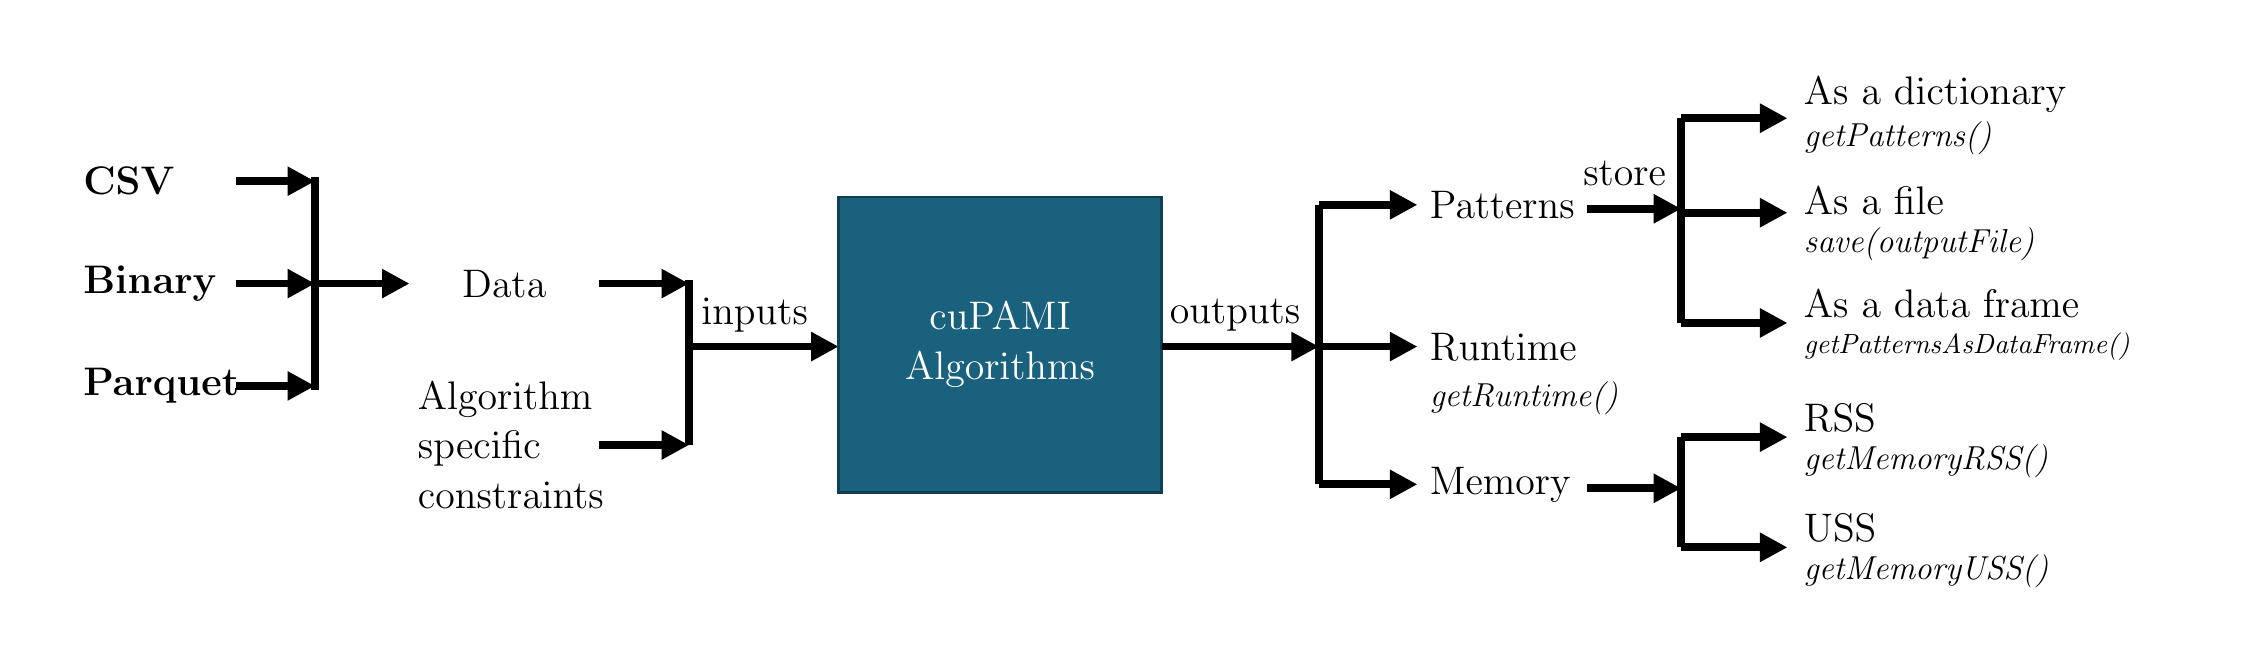
\begin{tikzpicture}[x=1cm,y=1cm,
 flow/.style={-{Triangle[length=3.5mm,width=3.5mm]},line width=2.8pt,draw=black},
 trunk/.style={line width=2.8pt,draw=black},
 txt/.style={anchor=west,align=left,font=\Large,inner sep=0pt},
 api/.style={anchor=west,font=\large\itshape,inner sep=0pt}]
% White canvas and plain input labels follow the reference diagram.
\fill[white] (0,0) rectangle (28,7.8);
\node[txt,text=black,font=\Large\bfseries] at (.7,5.85) {CSV};
\node[txt,text=black,font=\Large\bfseries] at (.7,4.55) {Binary};
\node[txt,text=black,font=\Large\bfseries] at (.7,3.25) {Parquet};
\draw[flow] (2.65,5.85) -- (3.65,5.85);
\draw[flow] (2.65,4.55) -- (3.65,4.55);
\draw[flow] (2.65,3.25) -- (3.65,3.25);
\draw[trunk] (3.65,3.2) -- (3.65,5.9);
\draw[flow] (3.65,4.55) -- (4.85,4.55);
\node[font=\Large,inner sep=0pt] at (6.05,4.55) {Data};
\draw[flow] (7.25,4.55) -- (8.4,4.55);
\node[txt] at (4.95,2.5) {Algorithm\\specific\\constraints};

\draw[flow] (7.25,2.5) -- (8.4,2.5);
\draw[trunk] (8.4,2.5) -- (8.4,4.6);
\node[txt] at (8.55,4.15) {inputs};
\draw[flow] (8.4,3.75) -- (10.3,3.75);
% Central square.
\filldraw[fill=teal,draw=teal!65!black,line width=1pt] (10.3,1.9) rectangle (14.4,5.65);
\node[text=white,align=center,font=\Large] at (12.35,3.775) {cuPAMI\\Algorithms};
% Outputs and their two secondary branches.
\node[txt] at (14.5,4.15) {outputs};
\draw[flow] (14.4,3.75) -- (16.4,3.75);
\draw[trunk] (16.4,2) -- (16.4,5.55);
\draw[flow] (16.4,5.55) -- (17.65,5.55);
\draw[flow] (16.4,3.75) -- (17.65,3.75);
\draw[flow] (16.4,2) -- (17.65,2);
\node[txt] at (17.8,5.55) {Patterns};
\node[txt] at (17.8,3.75) {Runtime};
\node[api] at (17.8,3.1) {getRuntime()};
\node[txt] at (17.8,2) {Memory};
\node[txt] at (19.75,5.95) {store};
\draw[flow] (19.8,5.5) -- (21,5.5);
\draw[trunk] (21,4.05) -- (21,6.65);
\draw[flow] (21,6.65) -- (22.35,6.65);
\draw[flow] (21,5.45) -- (22.35,5.45);
\draw[flow] (21,4.05) -- (22.35,4.05);
\node[txt] at (22.55,6.95) {As a dictionary};
\node[api] at (22.55,6.4) {getPatterns()};
\node[txt] at (22.55,5.6) {As a file};
\node[api] at (22.55,5.05) {save(outputFile)};
\node[txt] at (22.55,4.3) {As a data frame};
\node[anchor=west,font=\normalsize\itshape,inner sep=0pt] at (22.55,3.75) {getPatternsAsDataFrame()};
\draw[flow] (19.8,1.95) -- (21,1.95);
\draw[trunk] (21,1.2) -- (21,2.6);
\draw[flow] (21,2.6) -- (22.35,2.6);
\draw[flow] (21,1.2) -- (22.35,1.2);
\node[txt] at (22.55,2.85) {RSS};
\node[api] at (22.55,2.3) {getMemoryRSS()};
\node[txt] at (22.55,1.45) {USS};
\node[api] at (22.55,.9) {getMemoryUSS()};
\end{tikzpicture}
\end{document}
